\chapter{Introduction}
\label{ch:intro}
%-------------------------------------------------------
This report describes my implementation of the Scale-Invariant Feature Transform (SIFT) algorithm for extracting features and describing digital images. SIFT is a robust vision algorithm for salient point detection in the image that is insensitive to scaling, rotation, and illumination changes. For this project, I generated multiple versions of input images with different transformations and carried out the significant phases of the SIFT algorithm in an orderly manner: scale-space extrema detection, keypoint localization, and assignment of orientation. I monitored the algorithm's performance in different transformations of an image carefully in the process, noting down the intermediate outcomes at each step. My implementation used Python programming with the help of the OpenCV and NumPy libraries, which were found to be powerful tools for handling images as well as mathematical operations. In this report, I explain my procedural method, implementation decisions, experimental findings, and analysis of performance of the SIFT algorithm for feature detection and description in images.
%%%%%%
%%% SUBSECTION NAME
%%%%%%%%%%%%%%%%%%%%%%%%%%%%%%%%%%%%%%%%%%%%%%%%%%%%%
\chapter{Implementation}
\section{SIFT Implementation}
\subsection{First Step: Scale-space extrema detection}
The First step in SIFT is Scale-Space extrema implamentation. Using the openCV libary we can acually complete all of the SIFT Steps but than seperate them into the steps. OpenCV has built in SIFT functionality. Creating a SIFT object will allow us to complete the sift algorithm on a given image.
\begin{minted}[fontsize=\small, linenos, breaklines]{python}
sift = cv2.SIFT_create()

kp1, des1 = sift.detectAndCompute(img1, None)

img1Extrema = img1.copy()
\end{minted}

Once a SIFT Object is created we can extract all the steps from the keypoint features
To identify the Scale-Space Extrema we can simply plot the X,Y coordinates of the points to demonstrate the step of locating them
\begin{minted}[fontsize=\small, linenos, breaklines]{python}
for kp in kp1:
    x, y = kp.pt
    cv2.circle(img1Extrema, (int(x), int(y)), 2, (0, 0, 255), 2)

imageRightPhoto = ConvertCV2ToTKINTER(img1Extrema)
imageRight.config(image=imageRightPhoto)
imageRight.image = imageRightPhoto
\end{minted}

\begin{figure}[h!]
    \centering
    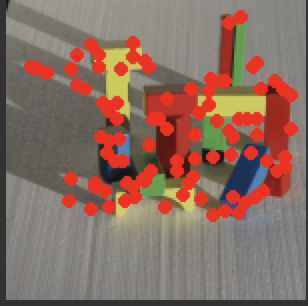
\includegraphics[width = .5\textwidth]{step1.png}
    \caption[First Step: Scale-space extrema detection]%
    {First Step: Scale-space extrema detection} 
    \label{fig:exG}
\end{figure}
\newpage

\subsection{Second Step: Keypoint localization}
Using the SIFT object from earlier we can extract the second step, by applying the frist step but also scaling the size of the circle that is directly propoertional to the key points scale
\begin{minted}[fontsize=\small, linenos, breaklines]{python}
 img1KeypointsScaled = img1.copy()
    for kp in kp1:
        x, y = kp.pt
        size = int(kp.size) 
        cv2.circle(img1KeypointsScaled, (int(x), int(y)), size, (0, 255, 255), 2)

    imageLeftMiddlePhoto = ConvertCV2ToTKINTER(img1KeypointsScaled)
    imageLeftMiddle.config(image=imageLeftMiddlePhoto)
    imageLeftMiddle.image = imageLeftMiddlePhoto
\end{minted}
\begin{figure}[h!]
    \centering
    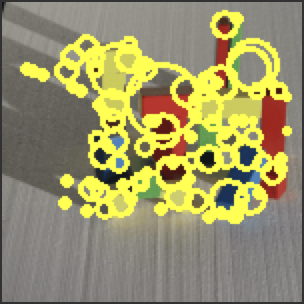
\includegraphics[width = .5\textwidth]{step2.png}
    \caption[Second Step: Keypoint localization]%
    {Second Step: Keypoint localization} 
    \label{fig:exa}
\end{figure}

\newpage

\subsection{Third Step: Orientation assignment}
Using the SIFT object from earlier we can assign the direction and orientation of the keypoints using the angle parameter of the keypoint object and Opencv build in arrowedLine functionality.
\begin{minted}[fontsize=\small, linenos, breaklines]{python}
    img1Orientation = img1.copy()
    for kp in kp1:
        x, y = kp.pt
        angle = np.deg2rad(kp.angle)
        length = kp.size / 2
        x2 = int(x + length * np.cos(angle))
        y2 = int(y + length * np.sin(angle))
        cv2.arrowedLine(img1Orientation, (int(x), int(y)), (x2, y2), (0, 255, 0), 1, tipLength=0.3)

    imageRightMiddlePhoto = ConvertCV2ToTKINTER(img1Orientation)
    imageRightMiddle.config(image=imageRightMiddlePhoto)
    imageRightMiddle.image = imageRightMiddlePhoto 
\end{minted}

\begin{figure}[h!]
    \centering
    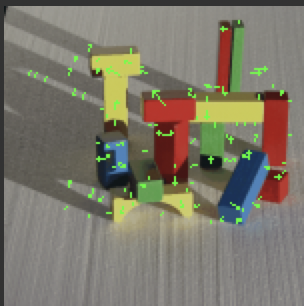
\includegraphics[width = .5\textwidth]{step3.png}
    \caption[Third Step: Orientation assignment]%
    {Third Step: Orientation assignment} 
    \label{fig:exB}
\end{figure}
\newpage

\subsection{Fourth Step: Keypoint descriptor}
For the fourth step, this is once again a parameter given by the openCV2 and we can print the descriptor arrays
these desscriptors are used to then match to other images that have similar keypoint descirptors. Using BF mathcing we can acutally attempt to match to different photos
\begin{minted}[fontsize=\small, linenos, breaklines]{python}
kp1, des1 = sift.detectAndCompute(img1, None)
Output:
\end{minted}
\centering
    \begin{tabular}{*{9}{c}}
        \hline
        17 & 0 & 0 & $\cdots$ & 14 & 4 & 0 \\
        30 & 23 & 10 & $\cdots$ & 2 & 0 & 1 \\
        31 & 2 & 0 & $\cdots$ & 7 & 2 & 0 \\
        $\vdots$ & $\vdots$ & $\vdots$ & $\ddots$ & $\vdots$ & $\vdots$ & $\vdots$ \\
        0 & 2 & 78 & $\cdots$ & 0 & 0 & 10 \\
        68 & 1 & 1 & $\cdots$ & 3 & 0 & 2 \\
        12 & 112 & 163 & $\cdots$ & 2 & 0 & 1 \\
        \hline
    \end{tabular}
    \label{tab:matrix-data}
\begin{figure}[h!]
    \centering
        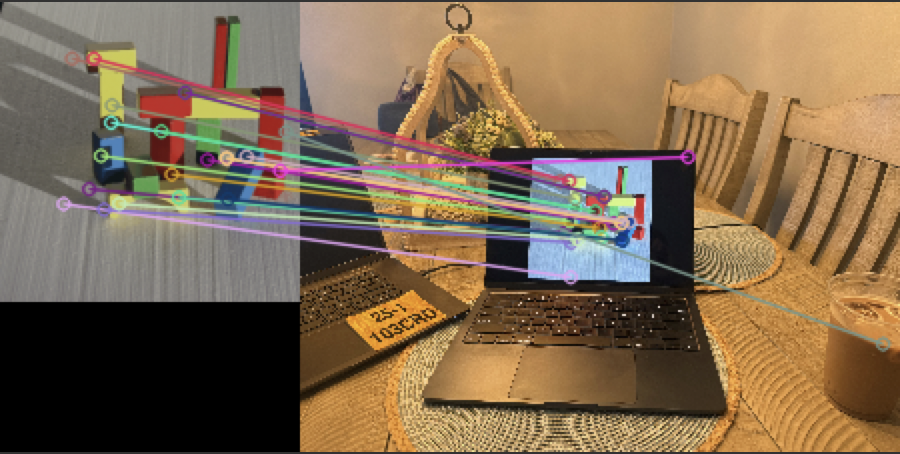
\includegraphics[width = .7\textwidth]{step4.png}
        \caption[Mathching]%
        {Mathching} 
        \label{fig:exC}
    \end{figure}

\newpage

\section{Results}
\begin{figure}[h!]
    \centering
        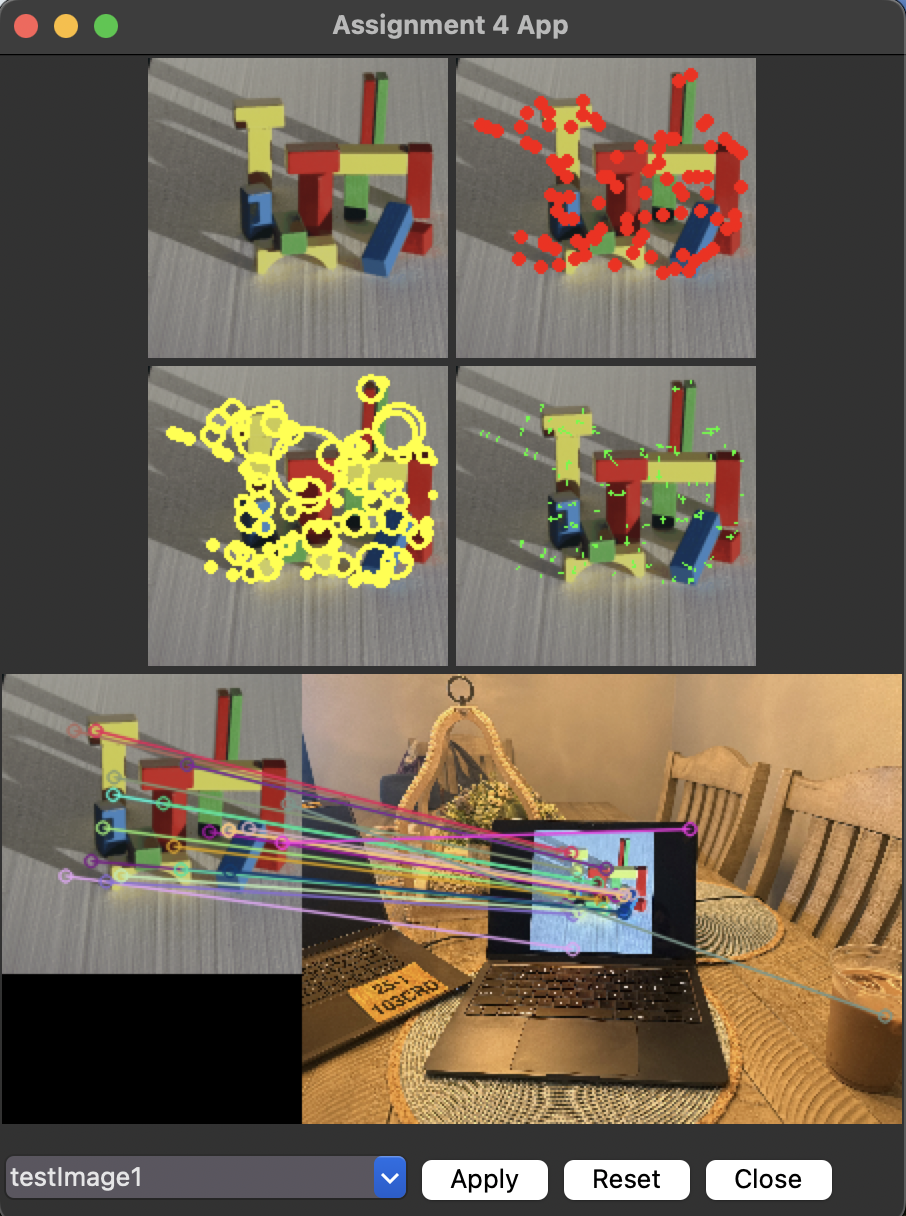
\includegraphics[width = .5\textwidth]{test1.png}
        \caption[Test 1]%
        {Test 1} 
        \label{fig:exD}
    \end{figure}
\newpage
\begin{figure}[h!]
    \centering
        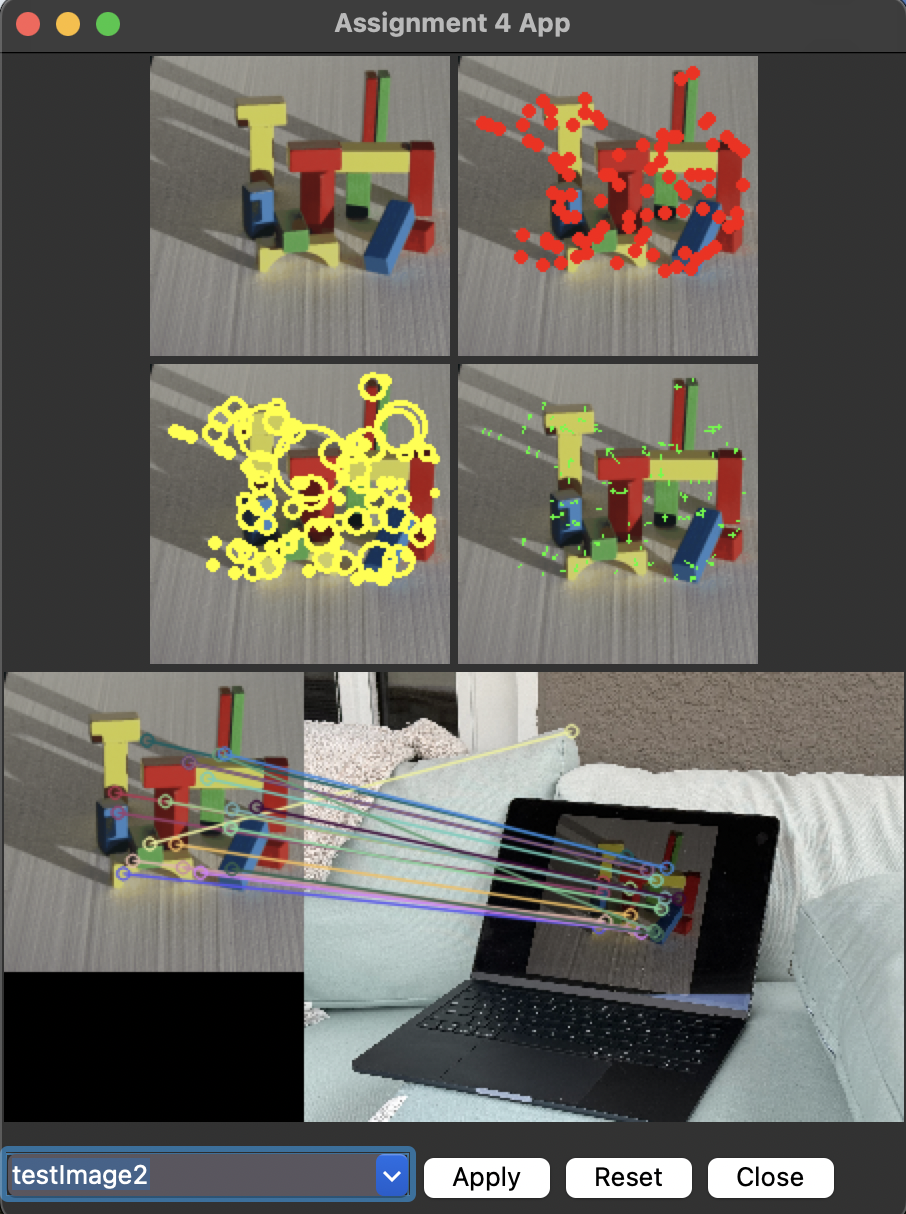
\includegraphics[width = .90\textwidth]{test2.png}
        \caption[Test 2]%
        {Test 2} 
        \label{fig:exE}
    \end{figure}
\newpage
\begin{figure}[h!]
    \centering
        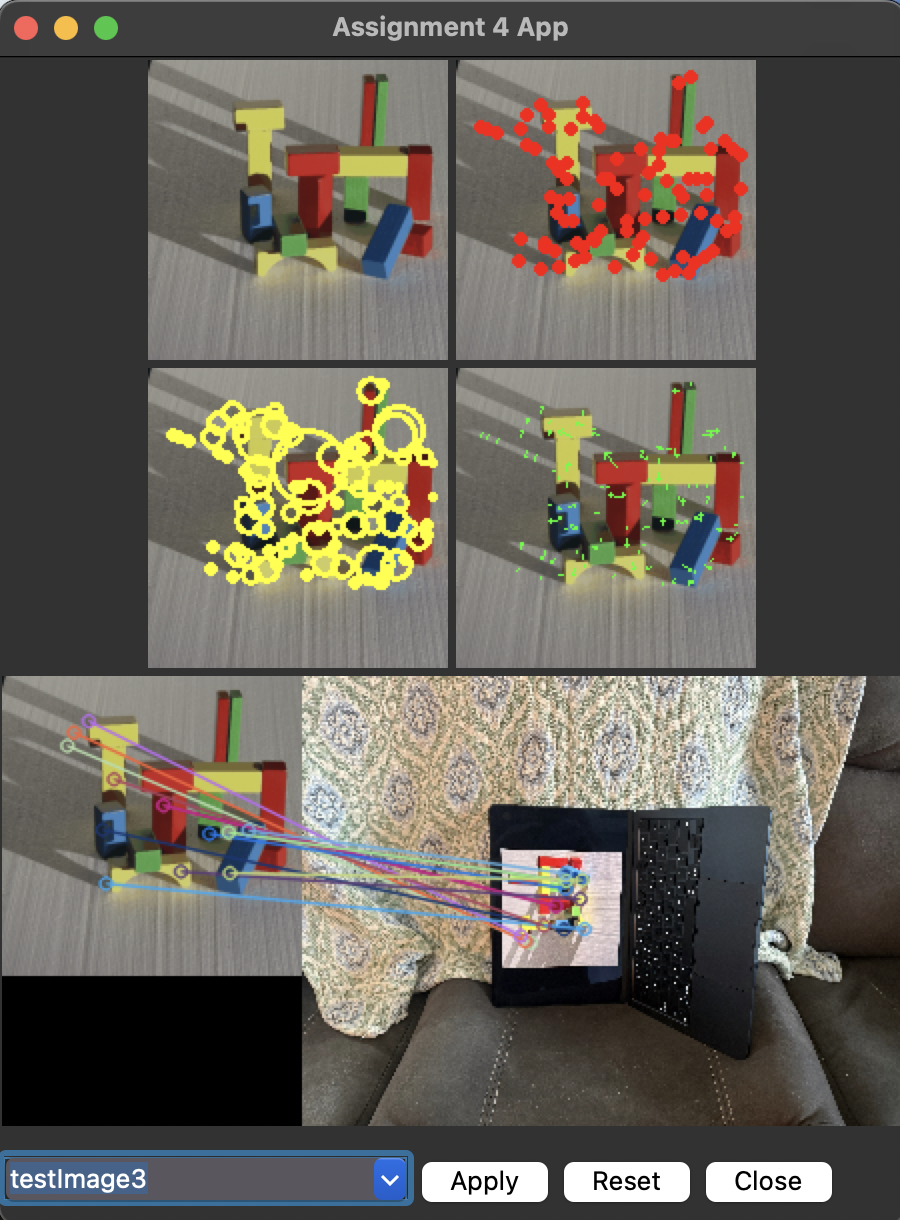
\includegraphics[width = .90\textwidth]{test3.png}
        \caption[Test 2]%
        {Test 2} 
        \label{fig:exF}
    \end{figure}
\newpage


%%%%%%%%%%%%%%%%%%
\newpage

\section{Discussion}
I applied the Scale-Invariant Feature Transform (SIFT) algorithm in detecting and describing features within various versions of an image. By detecting key points in varying sizes, their locations, and their directions, I established that SIFT detects significant features even as the size of the image, direction, or illumination varies. It was found through testing that this algorithm can detect the same key points within multiple copies of the same picture, demonstrating SIFT's largest asset as its capacity for detecting features that remain consistent.
Implementation revealed several significant aspects on how the algorithm functions. Building the scale-space pyramid was significant in detecting features of various sizes, and the use of the Difference of Gaussian (DoG) method worked well in approximating the Laplacian of Gaussian. The keypoint localization step enhanced the feature point quality since it discarded low-contrast points and responses of edges. Orientation assignment ensured there would be no effect due to rotation since it determined sizes of gradients as well as directions around each keypoint.
The project succeeded in meeting its overall objectives but has the potential for improvement in the future. In other words, this can be made faster for real-time applications, with an additional step for improved feature matching, and the ability for varying settings on achieving the appropriate amount and quality of keypoints for various applications. In summary, this project made me understand how feature detection algorithms function and how they are applied in object recognition, image matching, as well as in building 3D models.